%%%%%%%%%%%%%%%%%%%%%%%%%%%%%%%%%%%%%%%%%%%
%
% From a template maintained at https://github.com/jamesrobertlloyd/cbl-tikz-poster
%
% Code near the top should be fairly standard and not need to be changed
%  - except for the document class
% Code lower down is more likely to be customised
%
%%%%%%%%%%%%%%%%%%%%%%%%%%%%%%%%%%%%%%%%%%%

\pdfminorversion=4
\documentclass[landscape,a0b,final,a4resizeable]{include/a0poster}


\usepackage{multicol}
\usepackage{color}
\usepackage{morefloats}
\usepackage[pdftex]{graphicx}
\usepackage{rotating}
\usepackage{amsmath, amsthm, amssymb, bm}
\usepackage{array}
\usepackage{booktabs}
\usepackage{multirow}
\usepackage{hyperref}


\usepackage{include/picins}
\usepackage{tikz}
\usepackage{algorithm}% http://ctan.org/pkg/algorithms
\usepackage{algpseudocode}% http://ctan.org/pkg/algorithmicx
% \usepackage{algorithmic}
% \algsetup{linenosize=\small}
\usepackage{setspace}
\usepackage[hypcap=false,font=small,labelfont=bf]{caption} 
\usepackage{makecell}
\usetikzlibrary{shapes.geometric,arrows,chains,matrix,positioning,scopes,calc}
\tikzstyle{mybox} = [draw=white, rectangle]
\definecolor{darkblue}{rgb}{0,0.08,0.45}
\definecolor{blue}{rgb}{0,0,1}



\usepackage{nicefrac}
\newcommand{\vect}[1]{\underline{\smash{#1}}}
\renewcommand{\v}[1]{\vect{#1}}
\newcommand{\reals}{\mathds{R}}
\newcommand{\sX}{\mathcal{X}}
\newcommand{\sD}{\mathcal{D}}
\newcommand{\br}{}%{^{\text{\textnormal{ r}}}}
\newcommand{\cat}{^{\text{\textnormal{c}}}}

\usepackage{dsfont}

\ProvidesPackage{preamble}

\usepackage{url}
\usepackage{array}
\usepackage{amsmath,amssymb,amsfonts,textcomp,amsthm}
\usepackage{booktabs}
\usepackage{relsize}
\usepackage{nicefrac}
\usepackage{graphicx}
\usepackage{rotating}
\usepackage{nth}
\usepackage{acronym}
\usepackage{bm}
%\usepackage{caption} \DeclareCaptionType{copyrightbox}
\usepackage{footnote}
\usepackage{color}

\usepackage{tabularx}
\newcolumntype{x}[1]{>{\centering\arraybackslash\hspace{0pt}}m{#1}}
\newcommand{\tabbox}[1]{#1}

\usepackage{hyperref}
\definecolor{mydarkblue}{rgb}{0,0.08,0.45}
\hypersetup{
    pdftitle={},
    pdfauthor={},
    pdfsubject={},
    pdfkeywords={},
    pdfborder=0 0 0,
    pdfpagemode=UseNone,
    colorlinks=true,
    linkcolor=mydarkblue,
    citecolor=mydarkblue,
    filecolor=mydarkblue,
    urlcolor=mydarkblue,
    pdfview=FitH}

\newcommand{\asdf}{$^{\textnormal{th}}$}

\newcommand{\binarysum}{\sum_{\bf{x} \in \{0,1\}^D}}
\newcommand{\expect}{\mathbb{E}}
\newcommand{\expectargs}[2]{\mathbb{E}_{#1} \left[ {#2} \right]}
\newcommand{\var}{\mathbb{V}}
\newcommand{\varianceargs}[2]{\mathbb{V}_{#1} \left[ {#2} \right]}
\newcommand{\variance}{\mathbb{V}}
\newcommand{\cov}{\operatorname{cov}}
\newcommand{\Cov}{\operatorname{Cov}}
\newcommand{\covarianceargs}[2]{\Cov_{#1} \left[ {#2} \right]}
\newcommand{\colvec}[2]{\left[ \begin{array}{c} {#1} \\ {#2} \end{array} \right]}
\newcommand{\tbtmat}[4]{\left[ \begin{array}{cc} {#1} & {#2} \\ {#3} & {#4} \end{array} \right]}

%\newcommand{\covskinny}[2]{\var\!\left(#1\middle\vert#2\right)} 

\newcommand{\acro}[1]{\textsc{#1}}
%\newcommand{\vect}[1]{\boldsymbol{#1}}
%\newcommand{\vect}[1]{{\bf{#1}}}
\newcommand{\mat}[1]{\mathbf{#1}}
\newcommand{\pderiv}[2]{\frac{\partial #1}{\partial #2}}
\newcommand{\npderiv}[2]{\nicefrac{\partial #1}{\partial #2}}

\newcommand{\pha}{^{\phantom{:}}}

\newcommand{\argmin}{\operatornamewithlimits{argmin}}
\newcommand{\argmax}{\operatornamewithlimits{argmax}}

% The following designed for probabilities with long arguments

\newcommand{\Prob}[2]{P\!\left(\,#1\;\middle\vert\;#2\,\right)}
\newcommand{\ProbF}[3]{P\!\left(\,#1\!=\!#2\;\middle\vert\;#3\,\right)}
\newcommand{\p}[2]{p\!\left(#1\middle\vert#2\right)}
\newcommand{\po}[1]{p\!\left(#1\right)}
\newcommand{\pF}[3]{p\!\left(\,#1\!=\!#2\;\middle\vert\;#3\,\right)} 
\newcommand{\mean}[2]{{m}\!\left(#1\middle\vert#2\right)}
%\newcommand{\novmean}[2]{{m}\!\left(#1\middle\vert#2\right)}
%\newcommand{\novcov}[2]{\var\!\left(#1\middle\vert#2\right)}
%\newcommand{\cov}[2]{\var\!\left(#1\middle\vert#2\right)} 
%\newcommand{\pskinny}[2]{p\!\left(#1\;\middle\vert\;#2\right)}
%\newcommand{\meanskinny}[2]{{m}\!\left(#1\middle\vert#2\right)}
%\newcommand{\covskinny}[2]{\var\!\left(#1\middle\vert#2\right)} 

\newcommand{\vI}{\mat{I}}
\newcommand{\vX}{\mat{X}}
\newcommand{\vY}{\mat{Y}}
\newcommand{\vZ}{\mat{Z}}
\newcommand{\vK}{\mat{K}}
\newcommand{\vs}{\vect{s}}
\newcommand{\va}{\vect{a}}
\newcommand{\vA}{\vect{A}}
\newcommand{\vb}{\vect{b}}
\newcommand{\vB}{\mat{B}}
\newcommand{\vR}{\mat{R}}
\newcommand{\vS}{\mat{S}}
\newcommand{\vu}{\vect{u}}
\newcommand{\vk}{\vect{k}}
\newcommand{\vc}{\vect{c}}
\newcommand{\vC}{\mat{C}}
\newcommand{\vw}{\vect{w}}
\newcommand{\vx}{\vect{x}}
\newcommand{\vy}{\vect{y}}
\newcommand{\vz}{\vect{z}}
\newcommand{\vmu}{\vect{\mu}}
\newcommand{\vpi}{\vect{\pi}}
\newcommand{\vphi}{\vect{\phi}}
\newcommand{\vSigma}{\mat{\Sigma}}
\newcommand{\vtheta}{\vect{\theta}}
\newcommand{\vl}{\vect{l}}
\newcommand{\vq}{\vect{q}}
\newcommand{\vf}{\vect{f}}
\newcommand{\vg}{\vect{g}}
\newcommand{\vell}{\vect{\ell}}
\newcommand{\ve}{\vect{\epsilon}}
\newcommand{\vzero}{\vect{0}}
\newcommand{\vone}{\vect{1}}

\newcommand{\He}{\mathcal{H}}
\newcommand{\normx}[2]{\left\|#1\right\|_{#2}}
\newcommand{\Hnorm}[1]{\normx{#1}{\He}}
\newcommand{\mmd}{{\rm MMD}}


\newcommand{\mf}{\bar{\vf}}

\newcommand{\st}{_\star}

\newcommand{\inv}{^{{\mathsmaller{-1}}}}
\newcommand{\tohalf}{^{{\mathsmaller{\nicefrac{1}{2}}}}}

\newcommand{\Normal}{\mathcal{N}}
\newcommand{\N}[3]{\mathcal{N}\!\left(#1|#2,#3\right)}
\newcommand{\Nt}[2]{\mathcal{N}\!\left(#1,#2\right)}
\newcommand{\bN}[3]{\mathcal{N}\big(#1|#2,#3\big)}
\newcommand{\boldN}[3]{\text{\textbf{\mathcal{N}}}\big(#1;#2,#3\big)}
\newcommand{\ones}[1]{\mat{1}_{#1}}
\newcommand{\eye}[1]{\mat{E}_{#1}}
\newcommand{\tra}{{^\ensuremath{\mathsf{T}}}}
\newcommand{\trace}{\operatorname{tr}}
\newcommand{\deq}{:=}
\newcommand{\degree}{^\circ}

\newcommand{\GPt}[2]{\mathcal{GP}\!\left(#1,#2\right)}

\DeclareMathOperator{\chol}{chol}
\DeclareMathOperator{\diag}{diag}

\newcommand{\gp}{{\acro{gp}}}
\newcommand{\gplvm}{{\acro{gp-lvm}}}
\newcommand{\bmc}{{\acro{bmc}}}
\newcommand{\bq}{{\acro{bq}}}
\newcommand{\sbq}{{\acro{sbq}}}

\newenvironment{narrow}[2]{%
  \begin{list}{}{%
  \setlength{\topsep}{0pt}%
  \setlength{\leftmargin}{#1}%
  \setlength{\rightmargin}{#2}%
  \setlength{\listparindent}{\parindent}%
  \setlength{\itemindent}{\parindent}%
  \setlength{\parsep}{\parskip}}%
\item[]}{\end{list}}



\newcommand{\dist}{\ \sim\ }
\def\given{\,|\,}

% Table stuff
\newcolumntype{C}[1]{>{\centering\let\newline\\\arraybackslash\hspace{0pt}}m{#1}}
\newcolumntype{L}[1]{>{\raggedright\let\newline\\\arraybackslash\hspace{0pt}}m{#1}}
\newcolumntype{R}[1]{>{\raggedleft\let\newline\\\arraybackslash\hspace{0pt}}m{#1}}


\def\ie{i.e.\ }
\def\eg{e.g.\ }
\def\iid{i.i.d.\ }
%\def\simiid{\sim_{\mbox{\tiny iid}}}
\def\simiid{\overset{\mbox{\tiny iid}}{\sim}}
\def\eqdist{\stackrel{\mbox{\tiny d}}{=}}
\newcommand{\distas}[1]{\mathbin{\overset{#1}{\kern\z@\sim}}}

\def\Reals{\mathbb{R}}

\def\Uniform{\mbox{\rm Uniform}}
\def\Bernoulli{\mbox{\rm Bernoulli}}
\def\GP{\mathcal{GP}}
\def\GPLVM{\mathcal{GP-LVM}}

% Kernel stuff

\def\inputVar{x}
\def\InputVar{X}
\def\InputSpace{\mathcal{X}}
\def\outputVar{y}
\def\OutputSpace{\mathcal{Y}}
\def\function{f}
\def\kernel{k}
\def\KernelMatrix{K}
\def\SumKernel{\sum}
\def\ProductKernel{\prod}
\def\expression{e}

\def\SE{\acro{SE}}
\def\Per{\acro{Per}}
\def\RQ{\acro{RQ}}
\def\Lin{\acro{Lin}}

\def\subexpr{{\cal S}}
\def\baseker{{\cal B}}
\def\numWinners{k}

\newcommand{\kSE}{{\acro{SE}}}
\newcommand{\kPer}{{\acro{Per}}}
\newcommand{\kLin}{{\acro{Lin}}}
\newcommand{\kRQ}{{\acro{RQ}}}


% Proof stuff
\theoremstyle{plain}
\newtheorem{theorem}{Theorem}[section]
\newtheorem{lemma}[theorem]{Lemma}
\newtheorem{prop}[theorem]{Proposition}
\newtheorem*{cor}{Corollary}

%\input{include/preamble2.sty}

%\usepackage{tabularx}

%%%%%%%%%%%%%%%%%%%%%%%%%%%%%%%%%%%%%%%%%%%
%
% myfig
%
% \myfig - replacement for \figure
% necessary, since in multicol-environment 
% \figure won't work        
%                 
%%%%%%%%%%%%%%%%%%%%%%%%%%%%%%%%%%%%%%%%%%%

\newcommand{\myfig}[3][0]{
\begin{center}
  \vspace{1.5cm}
  \includegraphics[width=#3\hsize,angle=#1]{#2}
  \nobreak\medskip
\end{center}}

%%%%%%%%%%%%%%%%%%%%%%%%%%%%%%%%%%%%%%%%%%%
%
% mycaption                
%
% \mycaption - replacement for \caption
% necessary, since in multicol-environment \figure and
% therefore \caption won't work
%
%%%%%%%%%%%%%%%%%%%%%%%%%%%%%%%%%%%%%%%%%%%

%\newcounter{figure}
\setcounter{figure}{1}
\newcommand{\mycaption}[1]{
  \vspace{0.5cm}
  \begin{quote}
    {{\sc Figure} \arabic{figure}: #1}
  \end{quote}
  \vspace{1cm}
  \stepcounter{figure}
}

%%%%%%%%%%%%%%%%%%%%%%%%%%%%%%%%%%%%%%%%%%%
%
% Some standard colours
%
%%%%%%%%%%%%%%%%%%%%%%%%%%%%%%%%%%%%%%%%%%%

\definecolor{camlightblue}{rgb}{0.601 , 0.8, 1}
\definecolor{camdarkblue}{rgb}{0, 0.203, 0.402}
\definecolor{camred}{rgb}{1, 0.203, 0}
\definecolor{camyellow}{rgb}{1, 0.8, 0}
\definecolor{lightblue}{rgb}{0, 0, 0.80}
\definecolor{white}{rgb}{1, 1, 1}
\definecolor{whiteblue}{rgb}{0.80, 0.80, 1}

%%%%%%%%%%%%%%%%%%%%%%%%%%%%%%%%%%%%%%%%%%%
%
% Some look and feel definitions
%
%%%%%%%%%%%%%%%%%%%%%%%%%%%%%%%%%%%%%%%%%%%

\setlength{\columnsep}{0.03\textwidth}
\setlength{\columnseprule}{0.0018\textwidth}
\setlength{\parindent}{0.0cm}

%%%%%%%%%%%%%%%%%%%%%%%%%%%%%%%%%%%%%%%%%%%
%
% \mysection - replacement for \section*
% 
% Puts a pretty box around some text
% TODO - any other thoughts for what this box should look like
%
%%%%%%%%%%%%%%%%%%%%%%%%%%%%%%%%%%%%%%%%%%%

\tikzstyle{mysection} = [rectangle, 
									draw=none, 
									shade, 
									outer color=camlightblue!30,
									inner color=camlightblue!30,
									text width=0.965\columnwidth,
									text centered,
									rounded corners=20pt,
									minimum height=0.09\columnwidth]

\newcommand{\mysection}[1]
{
\begin{center}
  \begin{tikzpicture}
    \node[mysection] {\sffamily\bfseries\LARGE#1};
  \end{tikzpicture}
\end{center}
}

%%%%%%%%%%%%%%%%%%%%%%%%%%%%%%%%%%%%%%%%%%%
%
% Set the font
%
% TODO - Not sure what a canonical choice is - feel free to modify
%
%%%%%%%%%%%%%%%%%%%%%%%%%%%%%%%%%%%%%%%%%%%

\renewcommand{\familydefault}{cmss}
\sffamily

%%%%%%%%%%%%%%%%%%%%%%%%%%%%%%%%%%%%%%%%%%%%%%%%%%%%
%%%               Background                     %%%
%%%%%%%%%%%%%%%%%%%%%%%%%%%%%%%%%%%%%%%%%%%%%%%%%%%%

\newcommand{\background}[3]{
  %\definecolor{cgradbegin}{#1}
  %\definecolor{cgradend}{#2}
 % \psframe[fillstyle=gradient,gradend=cgradend,
 % gradbegin=cgradbegin,gradmidpoint=#3](0.,0.)(1.\textwidth,-1.\textheight)
}




%%%%%%%%%%%%%%%%%%%%%%%%%%%%%%%%%%%%%%%%%%%%%%%%%%%%
%%%                pcolumn                       %%%
%%%%%%%%%%%%%%%%%%%%%%%%%%%%%%%%%%%%%%%%%%%%%%%%%%%%

\newenvironment{pcolumn}[1]{
  \begin{minipage}{#1\textwidth}
  \begin{center}
}{
  \end{center}
  \end{minipage}
}



%%%%%%%%%%%%%%%%%%%%%%%%%%%%%%%%%%%%%%%%%%%%%%%%%%%%
%%%                pbox                          %%%
%%%%%%%%%%%%%%%%%%%%%%%%%%%%%%%%%%%%%%%%%%%%%%%%%%%%

\definecolor{lcolor}{rgb}{0, 0, 0.80}
\definecolor{gcolor1}{rgb}{1, 1, 1}
\definecolor{gcolor2}{rgb}{.80, .80, 1}

  % \def\fc{fillcolor}
  % \def\getfc #1=#2\par{\def\ffc{#1} \ifx\ffc\fc #2\fi} 
  % \def\getfillcolor #1,#2\par{\getfc #1\par \getfc #2\par}

 %  \newcommand{\psshadowbox}[2]{%[2][magenta]{
%      \fbox{Input arg: #1}
%      \fbox{#1} 
%      \fbox {\getfillcolor #1\par}
%      \def\col{\getfillcolor #1\par}
 
%      \let\coll=\col
%       \coll
 %     \colorbox{\col}{#2}
%       \mbox
   %   \coloredshadowbox{black}{\coll}{#2}
%   }

\newcommand{\pbox}[4]{
%\psshadowbox[#3]{
%\fbox{
\mbox{
\begin{minipage}[t][#2][t]{#1}
#4
\end{minipage}
}%}
}

%%%%%%%%%%%%%%%%%%%%%%%%%%%%%%%%%%%%%%%%%%%
%
% Poster environment
%
% Centres everything and can be used to define the width of the content
%
%%%%%%%%%%%%%%%%%%%%%%%%%%%%%%%%%%%%%%%%%%%

\newenvironment{poster}{
  \begin{center}
  \begin{minipage}[c]{\textwidth}
}{
  \end{minipage}
  \end{center}
}

\def\newarrow{\mbox{\begin{tikzpicture}
             \useasboundingbox{(-3pt,-4.5pt) rectangle (19pt,1pt)};
             \draw[->] (0,-0.07)--(17pt,-0.07);\end{tikzpicture}}}




\newcommand\transpose{{\textrm{\tiny{\sf{T}}}}}
\newcommand{\note}[1]{}
\newcommand{\hlinespace}{~\vspace*{-0.15cm}~\\\hline\\\vspace*{0.15cm}}
\newcommand{\embeddingletter}{g}
\newcommand{\bo}{{\sc bo}}
%\newcommand{\gp}{{\sc gp}}
\newcommand{\agp}{Arc \gp}



\begin{document}
\begin{poster}

% Potentially add some space at the top of the poster
\vspace{0\baselineskip}



%%% Header
\begin{center}
\begin{pcolumn}{0.99}

\newcommand{\logowidth}{0.06\textwidth}  % width mauna decomp

\pbox{0.99\textwidth}{}{linewidth=2mm,framearc=0.3,linecolor=camdarkblue,fillstyle=gradient,gradangle=0,gradbegin=white,gradend=white,gradmidpoint=1.0,framesep=1em}{
%%% U Toronto Logo
\hspace{2.3cm}
\begin{minipage}[c][][b]{\logowidth}
%  \begin{center}
    \vspace{-.18in}
    
\includegraphics[width=8cm,trim=9em 0em 9em 0em, clip]{badges/toronto}
   	% \hspace{35cm}
      
\includegraphics{badges/uot_text.png}
\end{minipage}
% \hspace{0.3cm}
% %
% %
% %%% Another Logo
% \begin{minipage}[c][][b]{\logowidth}
% %  \begin{center}
%     \vspace{.978in}
%     
\includegraphics[width=6cm]{badges/cambridgecrest}
%     
\includegraphics[width=6cm]{badges/unicamtext.pdf}
% %another 
% %  \end{center}
% \end{minipage}
%
%
%%% Title
\hspace{-5.0cm}
\begin{minipage}[c][9cm][c]{0.94\textwidth}
  \begin{center}
    \vspace{3.5cm}
    {\sffamily \VeryHuge \textbf{Generating Class-conditional Images\\\vspace{5.0mm} with Gradient-based Inference}}\\[10mm]
    {\huge\sffamily \Huge Bowen Xu, David Acuna, David Duvenaud\\[7.5mm]
    \Large \texttt{\{xubo3, davidj, duvenaud\}@cs.toronto.edu}
    }
  \end{center}
\end{minipage}
%
%
% % Harvard
% \begin{minipage}[c][][b]{\logowidth}
%   \begin{flushright}
% %    
\includegraphics[width=6cm,angle=0]{badges/cambridgecrest}
% %    \vspace{.1in}
% %    
\includegraphics[width=6cm,angle=0]{unicamtext.pdf}
%     
\includegraphics[width=8cm,trim=3.2em 0em 3.2em 3em, clip]{badges/harvard}
% %University of Cambridge 
%   \end{flushright}
% \end{minipage}
% %
% \hspace{1cm}
% 
% \begin{minipage}[c][][b]{\logowidth}
% %    
\includegraphics[width=6cm,angle=0]{badges/cambridgecrest}
% %    \vspace{.1in}
% %    
\includegraphics[width=6cm,angle=0]{unicamtext.pdf}
%     
\includegraphics[width=8cm,trim=0em 0em 0em 0em, clip]{badges/uni-freiburg}
% \end{minipage}
%
% \hspace{1cm}
% % 
% \begin{minipage}[c][][b]{\logowidth}
% %    
\includegraphics[width=6cm,angle=0]{badges/cambridgecrest}
% %    \vspace{.1in}
% %    
\includegraphics[width=6cm,angle=0]{unicamtext.pdf}
%     
\includegraphics[width=8cm,trim=0em 0em 0em 0em, clip]{badges/oxford}
% \end{minipage}

}
\end{pcolumn}
\end{center}

\vspace*{2.5cm}

\large


%%%%%%%%%%%%%%%%%%%%%%%%%%%%%%%%%%%%%%%%%%%%%%%%%%%%%%%%%%%%%%%%%%%%%%
%%% Begin of Document
%%%%%%%%%%%%%%%%%%%%%%%%%%%%%%%%%%%%%%%%%%%%%%%%%%%%%%%%%%%%%%%%%%%%%%


%%% Begin of Multicols-Enviroment
\begin{multicols}{3}
% 
\mysection{Main idea}
%
% 
\vspace{0.2in}
% 
% \begin{minipage}[c]{1\columnwidth}
\begin{itemize}
	\item Gradient descent on images is a promising approach to generating class-conditional images.
	\item This method produces high-resolution class-conditional images with crisp details and coherent overall structure.
	 %  often produces unrepresentative super-stimuli.
	\item Even better, we sample from $p(\textnormal{image} | \textnormal{class})$ using gradient-based MCMC methods.
	\item Our approach produces realistic and content-diverse class-conditional images.
	% \item The number of architecture-dependent hyperparameters changes with different architectures.
	\item Our method removes the need for \emph{ad-hoc} tweaks to the objective when longer iterations are introduced.
\end{itemize}
% \end{minipage}
% \begin{minipage}[c]{0.35\columnwidth}
% \begin{centering}
% \begin{tabular}{c}
% \input{tables/architecture-comparison} \\
% %\textcolor{darkblue}{ [Rasmussen, 1999]}
% \end{tabular}
% \end{centering}
% \end{minipage}

\vspace{0.5in}

\mysection{Previous Work}
% 
% approach, due to Nguyen et.\ al.\ \cite{Nguyen2016}, 
A previous approach due to Nguyen et.\ al.\ \cite{Nguyen2016} uses gradient-based optimization of images to do approximate 
% \emph{maximum a posteriori probability}
 MAP estimation, synthesizing large (227 x 227) class-conditional images.\\
% \begin{minipage}

\begin{center} 
  \centering
  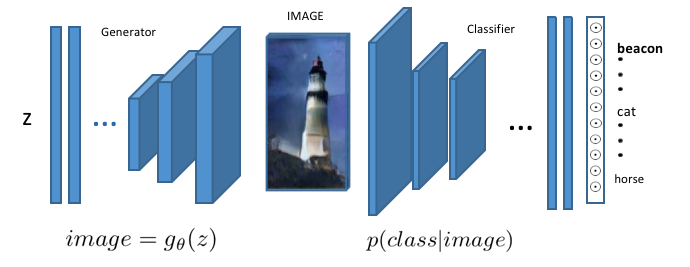
\includegraphics{figures/img}
  % \caption{Architecture using the DGN and DNN.}
  \label{fig:net}
\end{center}

\begin{itemize}
\item An initial image is specified by a random vector $z \thicksim \mathcal{N}(0, I)$.
 \item This vector is passed through a pre-trained image generation network $g_\theta(z)$.
\item The generated image is fed into a pre-trained classification network.
 \item The latent vector is then optimized using backpropagation.
 % according to the gradient of the chosen class probability with respect to the image, multiplied by the gradient of the image with respect to the latent vector, using backpropagation.
\end{itemize}
\vspace{1cm}
\mysection{Our contribution}
We use gradient-based MCMC methods to approximately sample from the class-conditional posterior:\\
\begin{equation*}
    \hat z \thicksim p(z|\textnormal{class}) \propto p(\textnormal{class} | g_\theta(z)) p(z) \qquad \textnormal{where} \qquad p(z) = \mathcal{N}(0, I)
    %\qquad \textnormal{where} \qquad p(z | class) = p(g_\theta(z) | class)
    % \label{eq:sampling}
\end{equation*}
\linebreak
and $p(\textnormal{class} | g_\theta(z))$ is the classification network.\\

We adopted:
\begin{itemize}
\item Hamiltonian Monte Carlo (HMC) 
\item Metropolis-adjusted-Langevin-algorithm (MALA) 
\end{itemize}
% \subsection*{Algorithm}
% \begin{algorithm}[H]
% % \setstretch{1.02}
%     % \caption{MAP with Clipping\cite{Nguyen2016}} %\label{evalgd}
%     \label{alg:activation_maximization}
%     \begin{algorithmic}[1]
%          \State $z \thicksim N(0,I)$
%          \For{ iterations }
%          \State $g= \nabla log(p(\textnormal{class}|z)p(z))$
%          \State \textbf{$z = z+\alpha g$}
%          \State $z= clip(z)$
%           \EndFor
%       \end{algorithmic}
% \end{algorithm}
% \vspace{-0.05in}
 

\newpage 

\mysection{Experiments and Results}
 \vspace{-0.05cm}
\begin{align*}
% % A simple figure to illustrate Mike and Frank's embedding
% Sept 2013

\newcommand{\scaleamount}{2.5}
\newcommand{\anglemin}{40}
\newcommand{\angleminplusone}{41}
\newcommand{\anglemax}{150}
\newcommand{\angleone}{70}
\newcommand{\angletwo}{120}
\newcommand{\bigradius}{3}
\newcommand{\biggerradius}{3.3}
\newcommand{\smallradius}{0.5}
\newcommand{\xtwolabelangle}{90}
\newcommand{\belowamount}{0.2cm}
\newcommand{\belowamounttwo}{0.11cm}
\newcommand{\myell}{l}
\newcommand{\embedding}{g}

%\begin{center}
%\framebox{
\begin{tikzpicture}
[trans/.style={thick,->,shorten >=2pt,shorten <=2pt,>=stealth},scale=\scaleamount]

\tikzset{state/.style={circle,draw=black, very thick,minimum size=4em}}

\def\centerarc[#1] (#2) (#3:#4:#5)% [draw options] (center) (initial angle:final angle:radius)
{ \draw[#1] (#2) ++(#3:#5) arc (#3:#4:#5);
}
	\coordinate (left) at ({\bigradius*cos(\anglemax)}, {\bigradius*sin(\anglemax)});
	\coordinate (right) at ({\bigradius*cos(\anglemin)}, {\bigradius*sin(\anglemin)});

	\coordinate (O1) at (-2, 0);
	\coordinate (O2) at (3, 1.25);
	
	\coordinate (left1) at ($ (left) + (O1) $);
	\coordinate (right1) at ($ (right) + (O1) $);
	\coordinate (left2) at ($ (left) + (O2) $);
	\coordinate (right2) at ($ (right) + (O2) $);
	
	% First arc
	% ==================
	
	% Draw arcs
	\centerarc[thick] (O1) (\anglemin:\anglemax:\bigradius)
	\centerarc[thick] (O1) (\anglemin:\anglemax:\smallradius)

	\draw[fill] (left1) circle (1.5pt);
	\draw (left1) node[below = \belowamount, right] {$\embedding(0, \textnormal{true}, u$)};
	
	\draw[fill] (right1) circle (1.5pt);
	\draw (right1) node[below = \belowamount] (r1below) {}
	               node[left] {$\embedding(0, \textnormal{true}, \myell)$};

	\draw[fill] (O1) circle (1.5pt);
	\draw (O1) node[below = \belowamount] (o1below) {}
	           node[left = 0.3cm] {$\embedding(0, \textnormal{false}, \cdot)$};

	\draw (left1) -- (O1) node[above] {$\rho \pi$};
	\draw (right1) -- (O1) node[midway, below] {$\omega$};
	
	
	% Second arc
	% ================================
	\centerarc[thick] (O2) (\anglemin:\anglemax:\bigradius)
	\centerarc[thick] (O2) (\anglemin:\anglemax:\smallradius)

	\draw[fill] (left2) circle (1.5pt);
	
	\draw[fill] (right2) circle (1.5pt);
	\draw (right2) node[below = \belowamount] (r2below) {};
	

	\draw[fill] (O2) circle (1.5pt);
	\draw (O2) node[below = \belowamount] (o2below) {}
                   node[right] {$\embedding(1, \textnormal{false}, \cdot)$};

	\draw[dashed] (left2) -- (O2);
	\draw[dashed] (right2) -- (O2);


	% Connect the arcs
	\draw (left1) -- (left2);
	\draw (right1) -- (right2);
	\draw[thick] (O1) -- (O2);
	
	% Draw surface
	\foreach \i in {\angleminplusone, ..., \anglemax}
	{
		\coordinate (arca) at ({\bigradius*cos(\i)}, {\bigradius*sin(\i)});
		\coordinate (arcb) at ({\bigradius*cos(\i - 1)}, {\bigradius*sin(\i - 1)});
		\coordinate (arca1) at ($ (arca) + (O1) $);
		\coordinate (arca2) at ($ (arca) + (O2) $);
		\coordinate (arcb1) at ($ (arcb) + (O1) $);
		\coordinate (arcb2) at ($ (arcb) + (O2) $);
%		\draw[green] (arca1) -- (arca2);
		\fill[fill=blue!40,fill opacity=0.8](arca1)--(arca2)--(arcb2)--(arcb1)--cycle;
	}

	\draw (right2) node[left] {$\embedding(1, \textnormal{true}, \myell)$};

	% Draw arrows showing in which direction x1 varies.
	\coordinate(x1half) at ($ (right1)!0.5!(right2) $);
	\draw (x1half) node[below = \belowamounttwo] (x1halfbelow) {$x_1$};
	\draw[trans] ($ (r1below)!0.45!(r2below) $) -- ($ (r1below)!0.3!(r2below) $);
	\draw[trans] ($ (r1below)!0.55!(r2below) $) -- ($ (r1below)!0.7!(r2below) $);

	\coordinate(x2half) at ($ (O1)!0.6!(O2) $);
	\draw (x2half) node[below = \belowamounttwo] (x2halfbelow) {$x_1$};
	\draw[trans] ($ (o1below)!0.55!(o2below) $) -- ($ (o1below)!0.4!(o2below) $);
	\draw[trans] ($ (o1below)!0.65!(o2below) $) -- ($ (o1below)!0.8!(o2below) $);

	% Draw arrows showing in which direction x2 varies.
	\coordinate (arclabel) at ($ (O1) + ({\biggerradius*cos(\xtwolabelangle)}, {\biggerradius*sin(\xtwolabelangle)}) $);
	\draw (arclabel) node {$x_2$};
	\centerarc[trans] (O1) ( \xtwolabelangle + 5  :  \xtwolabelangle + 30  :\biggerradius)
	\centerarc[trans] (O1) ( \xtwolabelangle - 5  :  \xtwolabelangle - 30  :\biggerradius)

%	\coordinate (x1) at ({\bigradius*cos(\angletwo)}, {\bigradius*sin(\angletwo)});
%	\coordinate (x2) at ({\bigradius*cos(\angleone)}, {\bigradius*sin(\angleone)});
%	\draw[fill] (x1) circle (1.5pt);
%	\draw (x1) node[above, left] {$f(x_1, \textnormal{true})$};
%	\draw[fill] (x2) circle (1.5pt);
%	\draw (x2) node[above, right] {$f(x_2, \textnormal{true})$};
\end{tikzpicture}
%}
%\end{center}
\label{fig:cylinder}
% \begin{figure}[h]
  % \centering
  %\includegraphics[width=\textwidth]{ComparisonImagebyImage_wo_clipping}
  \hspace{-2.0cm}
  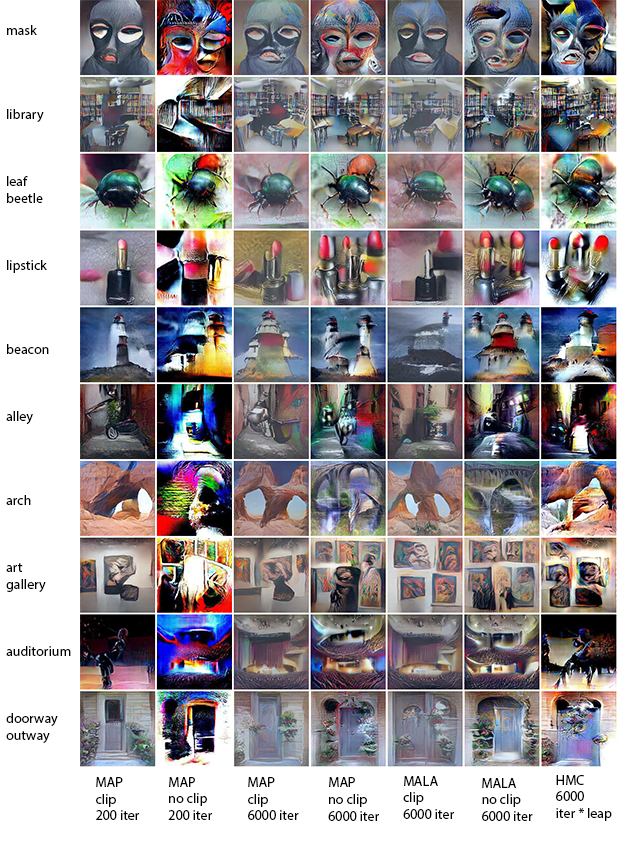
\includegraphics[width=32cm,keepaspectratio=false]{figures/comparison_final_transpose}
  % [scale=0.5725]
  % \caption{Images generated with MAP, MALA, and HMC.}
  % \label{fig:robustness}
\end{align*}
% 
\mysection{Automatically Evaluating Image Quality}

We use a discriminator \cite{Radford2015}, trained on ImageNet, to output the probability of an image being natural versus synthesized.\\

\begin{minipage}[c]{1\columnwidth}
        \centering
        \resizebox{\textwidth}{!}{
        \begin{tabular}{ ccccc}
            %\hline
              & \makecell{MAP with\\ class-specific regularization}  & \makecell{MALA with\\ class-specific regularization} & MALA & HMC\\
            \midrule 
            Average log-probability & -6.00 & {\bf -5.53} & -9.79 & -7.96
		\end{tabular}}
        % \caption{Average log-probability of synthetic images being real.}
        \label{table:dt_test}
\end{minipage}



\newpage
\mysection{Diversity of Image Contents}
\vspace{-0.5cm}
\begin{align*}
% % A simple figure to illustrate Mike and Frank's embedding
% Sept 2013

\newcommand{\scaleamount}{2.5}
\newcommand{\anglemin}{40}
\newcommand{\angleminplusone}{41}
\newcommand{\anglemax}{150}
\newcommand{\angleone}{70}
\newcommand{\angletwo}{120}
\newcommand{\bigradius}{3}
\newcommand{\biggerradius}{3.3}
\newcommand{\smallradius}{0.5}
\newcommand{\xtwolabelangle}{90}
\newcommand{\belowamount}{0.2cm}
\newcommand{\belowamounttwo}{0.11cm}
\newcommand{\myell}{l}
\newcommand{\embedding}{g}

%\begin{center}
%\framebox{
\begin{tikzpicture}
[trans/.style={thick,->,shorten >=2pt,shorten <=2pt,>=stealth},scale=\scaleamount]

\tikzset{state/.style={circle,draw=black, very thick,minimum size=4em}}

\def\centerarc[#1] (#2) (#3:#4:#5)% [draw options] (center) (initial angle:final angle:radius)
{ \draw[#1] (#2) ++(#3:#5) arc (#3:#4:#5);
}
	\coordinate (left) at ({\bigradius*cos(\anglemax)}, {\bigradius*sin(\anglemax)});
	\coordinate (right) at ({\bigradius*cos(\anglemin)}, {\bigradius*sin(\anglemin)});

	\coordinate (O1) at (-2, 0);
	\coordinate (O2) at (3, 1.25);
	
	\coordinate (left1) at ($ (left) + (O1) $);
	\coordinate (right1) at ($ (right) + (O1) $);
	\coordinate (left2) at ($ (left) + (O2) $);
	\coordinate (right2) at ($ (right) + (O2) $);
	
	% First arc
	% ==================
	
	% Draw arcs
	\centerarc[thick] (O1) (\anglemin:\anglemax:\bigradius)
	\centerarc[thick] (O1) (\anglemin:\anglemax:\smallradius)

	\draw[fill] (left1) circle (1.5pt);
	\draw (left1) node[below = \belowamount, right] {$\embedding(0, \textnormal{true}, u$)};
	
	\draw[fill] (right1) circle (1.5pt);
	\draw (right1) node[below = \belowamount] (r1below) {}
	               node[left] {$\embedding(0, \textnormal{true}, \myell)$};

	\draw[fill] (O1) circle (1.5pt);
	\draw (O1) node[below = \belowamount] (o1below) {}
	           node[left = 0.3cm] {$\embedding(0, \textnormal{false}, \cdot)$};

	\draw (left1) -- (O1) node[above] {$\rho \pi$};
	\draw (right1) -- (O1) node[midway, below] {$\omega$};
	
	
	% Second arc
	% ================================
	\centerarc[thick] (O2) (\anglemin:\anglemax:\bigradius)
	\centerarc[thick] (O2) (\anglemin:\anglemax:\smallradius)

	\draw[fill] (left2) circle (1.5pt);
	
	\draw[fill] (right2) circle (1.5pt);
	\draw (right2) node[below = \belowamount] (r2below) {};
	

	\draw[fill] (O2) circle (1.5pt);
	\draw (O2) node[below = \belowamount] (o2below) {}
                   node[right] {$\embedding(1, \textnormal{false}, \cdot)$};

	\draw[dashed] (left2) -- (O2);
	\draw[dashed] (right2) -- (O2);


	% Connect the arcs
	\draw (left1) -- (left2);
	\draw (right1) -- (right2);
	\draw[thick] (O1) -- (O2);
	
	% Draw surface
	\foreach \i in {\angleminplusone, ..., \anglemax}
	{
		\coordinate (arca) at ({\bigradius*cos(\i)}, {\bigradius*sin(\i)});
		\coordinate (arcb) at ({\bigradius*cos(\i - 1)}, {\bigradius*sin(\i - 1)});
		\coordinate (arca1) at ($ (arca) + (O1) $);
		\coordinate (arca2) at ($ (arca) + (O2) $);
		\coordinate (arcb1) at ($ (arcb) + (O1) $);
		\coordinate (arcb2) at ($ (arcb) + (O2) $);
%		\draw[green] (arca1) -- (arca2);
		\fill[fill=blue!40,fill opacity=0.8](arca1)--(arca2)--(arcb2)--(arcb1)--cycle;
	}

	\draw (right2) node[left] {$\embedding(1, \textnormal{true}, \myell)$};

	% Draw arrows showing in which direction x1 varies.
	\coordinate(x1half) at ($ (right1)!0.5!(right2) $);
	\draw (x1half) node[below = \belowamounttwo] (x1halfbelow) {$x_1$};
	\draw[trans] ($ (r1below)!0.45!(r2below) $) -- ($ (r1below)!0.3!(r2below) $);
	\draw[trans] ($ (r1below)!0.55!(r2below) $) -- ($ (r1below)!0.7!(r2below) $);

	\coordinate(x2half) at ($ (O1)!0.6!(O2) $);
	\draw (x2half) node[below = \belowamounttwo] (x2halfbelow) {$x_1$};
	\draw[trans] ($ (o1below)!0.55!(o2below) $) -- ($ (o1below)!0.4!(o2below) $);
	\draw[trans] ($ (o1below)!0.65!(o2below) $) -- ($ (o1below)!0.8!(o2below) $);

	% Draw arrows showing in which direction x2 varies.
	\coordinate (arclabel) at ($ (O1) + ({\biggerradius*cos(\xtwolabelangle)}, {\biggerradius*sin(\xtwolabelangle)}) $);
	\draw (arclabel) node {$x_2$};
	\centerarc[trans] (O1) ( \xtwolabelangle + 5  :  \xtwolabelangle + 30  :\biggerradius)
	\centerarc[trans] (O1) ( \xtwolabelangle - 5  :  \xtwolabelangle - 30  :\biggerradius)

%	\coordinate (x1) at ({\bigradius*cos(\angletwo)}, {\bigradius*sin(\angletwo)});
%	\coordinate (x2) at ({\bigradius*cos(\angleone)}, {\bigradius*sin(\angleone)});
%	\draw[fill] (x1) circle (1.5pt);
%	\draw (x1) node[above, left] {$f(x_1, \textnormal{true})$};
%	\draw[fill] (x2) circle (1.5pt);
%	\draw (x2) node[above, right] {$f(x_2, \textnormal{true})$};
\end{tikzpicture}
%}
%\end{center}
\label{fig:cylinder}
% \begin{figure}[h]
% 
  %\includegraphics[width=\textwidth]{ComparisonImagebyImage_wo_clipping}
   % \hspace{-1.0cm}
   % \hspace{0.8cm}
  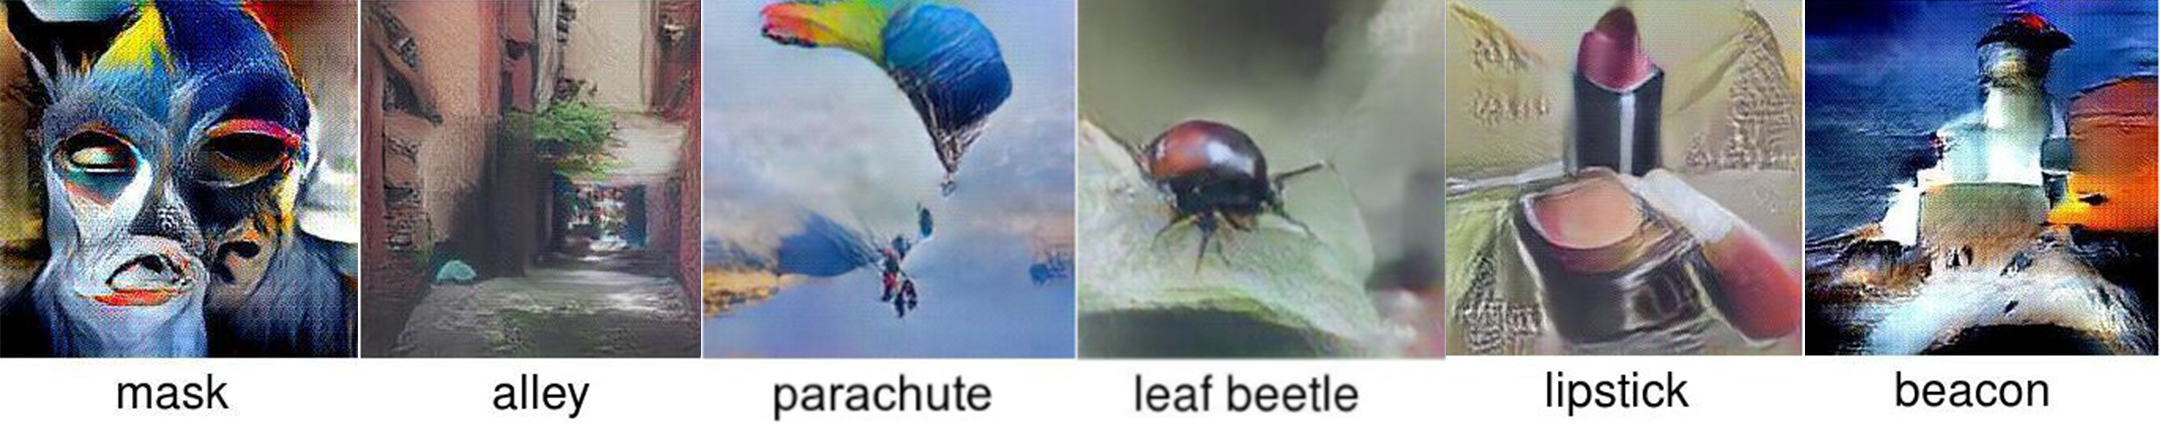
\includegraphics[width=33cm,keepaspectratio=false]{figures/moreRepresentative}
  % [scale=0.5725]
  % \caption{Images generated with MAP, MALA, and HMC.}
  % \label{fig:robustness}
\end{align*}



\mysection{Advantages and Limitations}
\begin{itemize}
	\setlength\itemsep{0.4em}
	\item[$+$] Produces high-resolution images with crisp details and coherent overall structure.
	\item[$+$] Generates more content-diverse images.
	\item[$+$] Removes the need for class-specific regularization when longer iterations are introduced.
	% \item[$+$] If longer iterations are introduced clipping constraints are not required.
	% \item[$-$] Slow convergence for high-dimensional data spaces.
	\item[$-$] Small step sizes and longer iterations are required.
\end{itemize}
% \begin{minipage}[c]{0.95\columnwidth}
% %\begin{table}[h!]
% %\caption{{\small \label{tab:nn_error}}}
% %\label{tbl:nn_nmse}
% \input{tables/mcmc-table.tex}
 



\vspace{1.cm}
\mysection{Future Work}
	\begin{itemize}
		\setlength\itemsep{0.4em}
		\item Use the Hamiltonian Variational Inference (HVI) model \cite{2014arXiv1410.6460S}.
		\item Generate images from text.
		\item Generate other media such as sound and video.
 	\end{itemize}
% %\begin{figure}[t!]
% 	\centering
% %	\begin{subfigure}[]{0.3\textwidth}
% \begin{tabular}{cc}
% \includegraphics[width=0.45\columnwidth]{figures/mnist.pdf} &
% \includegraphics[width=0.45\columnwidth]{figures/cifar10.pdf} \\
% MNIST &  CIFAR-10
% \end{tabular}		


% \begin{tabular}{c}
% 		\includegraphics[width=0.45\columnwidth]{figures/fevals_per_layer.pdf} \\
% Architectures searched
% \end{tabular}
		
%		\label{fig:proparchs}
%	\end{subfigure}
%	\caption{Bayesian optimization results using the arc kernel.}
%	\label{fig:arcbo}
%\vspace{-0.3cm}
%\end{figure}

\vspace{1.cm}
% \hspace{-1.0cm}

\mysection{Bibliography}
\small
\begingroup
\renewcommand{\section}[2]{}%
\bibliography{bib}
\endgroup
\bibliographystyle{ieeetr}

\vspace{1.5cm}
 \begin{center}
\begin{minipage}[c]{0.2\columnwidth}
  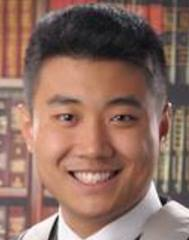
\includegraphics[width=8cm]{photos/xu}
  \captionsetup{labelformat=empty}
  \captionof{figure}{Bowen Xu}
\end{minipage}
\hspace{0.5cm}
\begin{minipage}[c]{0.2\columnwidth}
  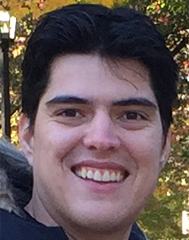
\includegraphics[width=8cm]{photos/acuna}
  \captionsetup{labelformat=empty}
  \captionof{figure}{David Acuna}
\end{minipage}
\hspace{0.5cm}
\begin{minipage}[c]{0.2\columnwidth}
  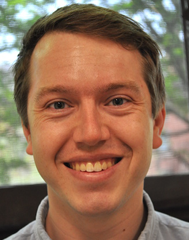
\includegraphics[width=8cm]{photos/duvenaud.png}
  \captionsetup{labelformat=empty}
  \captionof{figure}{David Duvenaud}
\end{minipage}
\end{center}
 
%\paragraph{Code}
%Code available at \texttt{http://???}
%
%Paper available at \texttt{http://???}
 

\end{multicols}
\end{poster}
\end{document}

